%!TEX root = ./paper.tex
\usepackage{cleveref}
\usepackage{subcaption}
\usepackage{adjustbox}
\usepackage{graphicx}
\usepackage{xcolor}

\definecolor {codeBackground} {HTML} {F4F4F4} % {F7F7F7} AYU common.bg
\definecolor {codeForeground} {HTML} {000000} % AYU common.fg
\definecolor {codeKeyword}    {HTML} {399EE6} % AYU syntax.entity
\definecolor {codeBuiltin}    {HTML} {55B4D4} % AYU syntax.tag
\definecolor {codeConstant}   {HTML} {A37ACC} % AYU syntax.constant
\definecolor {codeString}     {HTML} {86B300} % AYU syntax.string
\definecolor {codeEmph}       {HTML} {FA8D3E} % AYU syntax.keyword
\definecolor {codeRuler}      {HTML} {CACACA} % AYU ui.panel.border
\definecolor {codeComment}    {HTML} {8A9199} % AYU common.ui
\definecolor {codeIdentifier} {HTML} {1c1c1c}
\definecolor {codeOperator}   {HTML} {4CBF99}
\definecolor {codeError}      {HTML} {E65050} % AYU common.error

\usepackage[flushleft,alwaysadjust]{paralist}
\AtBeginDocument{\setdefaultleftmargin{0.7em}{}{}{}{}{}}

\crefname{option}{option}{options}
\Crefname{option}{Option}{Options}

\usepackage{relsize}
\usepackage{twemojis}
\usepackage{fancyvrb}
\usepackage{listings}
\lstset{
  inputencoding=utf8,
  basicstyle=\ttfamily\mdseries,
  fancyvrb=true,
  sensitive=true,
  numberstyle=\smaller[2]\ttfamily\color{codeRuler},
  numberblanklines=false,
  %breaklines=true,
  extendedchars=false, showstringspaces=false, columns=fixed, stepnumber=1,
  escapeinside={\%*}{*)}, lineskip=-5pt, basewidth=0.5em }

\definecolor{pc}{HTML}{55B4D4}
\definecolor{branching}{HTML}{FA8D3E}
\definecolor{arithmetic}{HTML}{ED9366}
\definecolor{stack}{HTML}{A37ACC}
\definecolor{userio}{HTML}{4CBF99}
\definecolor{gridio}{HTML}{86B300}
\definecolor{stringmode}{HTML}{FF7383}
\definecolor{endprogram}{HTML}{E65050}
\definecolor{ignore}{HTML}{787B80}
\definecolor{number}{HTML}{5C6166}
\definecolor{codebg}{HTML}{F3F4F5}

\colorlet{stringbg}{stringmode!20}
\colorlet{pcbg}{pc!20}
\colorlet{branchingbg}{branching!20}

\newcommand{\keyword}[1]{{\color{codeKeyword}\bfseries\ttfamily #1}}

\lstdefinelanguage{sql}{
basicstyle=\linespread{1.0}\color{codeForeground}\ttfamily\mdseries,
identifierstyle=\color{codeIdentifier},
commentstyle=\color{codeComment},
stringstyle=\color{codeString},
emphstyle={\color{codeEmph}\itshape\bfseries},
keywordstyle={[1]\color{codeKeyword}\bfseries},
keywordstyle={[2]\color{codeBuiltin}\bfseries},
keywordstyle={[3]\color{codeConstant}\bfseries},
keywordstyle={[4]\color{codeOperator}\bfseries},
emptylines=*10,
morestring=[d]{'},
morecomment=[l]{--},
morekeywords=[1]{WITH,RECURSIVE,UNION,ALL,SELECT,FROM,WHERE,CASE,WHEN,THEN,END,LATERAL,AS,ITERATE,LEFT,RIGHT,OUTER,INNER,JOIN,IF,ELSE,ELSIF},
morekeywords=[2]{int4,float8,text,boolean,ARRAY,CARDINALITY,ABS,FLOOR,CEIL,ROUND,RANDOM,SIGN,MAX,MIN,ARRAY_AGG,unnest,json_each},
morekeywords=[3]{NULL,TRUE,FALSE},
morekeywords=[4]{AND,OR,NOT,BETWEEN,IS},
literate=%
{(}{{{\color{codeOperator}(}}}1
    {)}{{{\color{codeOperator})}}}1
{[}{{{\color{codeOperator}[}}}1
{]}{{{\color{codeOperator}]}}}1
% {\{}{{{\color{codeOperator}\{}}1
% {\}}{{{\color{codeOperator}\}}}1
{:}{{{\color{codeOperator}:}}}1
{.}{{{\color{codeOperator}.}}}1
{,}{{{\color{codeOperator},}}}1
{+}{{{\color{codeOperator}+}}}1
{-}{{{\color{codeOperator}-}}}1
{*}{{{\color{codeOperator}*}}}1
{/}{{{\color{codeOperator}/}}}1
{\%}{{{\color{codeOperator}\%{}}}}1
{@}{{{\color{codeOperator}@}}}1
{^}{{{\color{codeOperator}\^{}}}}1
{|}{{{\color{codeOperator}|}}}1
{\&}{{{\color{codeOperator}\&}}}1
{<}{{{\color{codeOperator}<}}}1
{>}{{{\color{codeOperator}>}}}1
{=}{{{\color{codeOperator}=}}}1
{!}{{{\color{codeOperator}!}}}1
{...}{{{\color{codeComment}...}}}3
}
\newcommand{\sql}[1]{\text{\lstinline[language=sql]!#1!}}

\lstdefinelanguage{py}{
basicstyle=\linespread{1.0}\color{codeForeground}\ttfamily,
identifierstyle=\color{codeIdentifier},
commentstyle=\color{codeComment},
stringstyle=\color{codeString},
emphstyle={\color{codeEmph}\itshape\bfseries},
keywordstyle={[1]\color{codeKeyword}\bfseries},
keywordstyle={[2]\color{codeBuiltin}\bfseries},
keywordstyle={[3]\color{codeConstant}\bfseries},
keywordstyle={[4]\color{codeOperator}\bfseries},
emptylines=*10,
morestring=[d]{"},
morecomment=[l]{\#},
morekeywords=[1]{def,for,while,if,else,try,except,finally,yield,async,await,return,match,case,switch,do},
morekeywords=[2]{int,float,bool,str,list,dict,set},
morekeywords=[3]{None,True,False},
morekeywords=[4]{is,not,in,and,or},
literate=%
{(}{{{\color{codeOperator}(}}}1
    {)}{{{\color{codeOperator})}}}1
{[}{{{\color{codeOperator}[}}}1
{]}{{{\color{codeOperator}]}}}1
% {\{}{{{\color{codeOperator}\{}}1
% {\}}{{{\color{codeOperator}\}}}1
{:}{{{\color{codeOperator}:}}}1
{.}{{{\color{codeOperator}.}}}1
{,}{{{\color{codeOperator},}}}1
{+}{{{\color{codeOperator}+}}}1
{-}{{{\color{codeOperator}-}}}1
{*}{{{\color{codeOperator}*}}}1
{/}{{{\color{codeOperator}/}}}1
{\%}{{{\color{codeOperator}\%{}}}}1
{@}{{{\color{codeOperator}@}}}1
{^}{{{\color{codeOperator}\^{}}}}1
{|}{{{\color{codeOperator}|}}}1
{\&}{{{\color{codeOperator}\&}}}1
{<}{{{\color{codeOperator}<}}}1
{>}{{{\color{codeOperator}>}}}1
{==}{{{\color{codeOperator}==}}}2
{!=}{{{\color{codeOperator}!=}}}2
{<=}{{{\color{codeOperator}<=}}}2
{>=}{{{\color{codeOperator}>=}}}2
{...}{{{\color{codeComment}...}}}3
{=}{{{\color{codeConstant}=}}}1
}
\newcommand{\py}[1]{\text{\lstinline[language=py]!#1!}}

\lstdefinelanguage{befunge}{
basicstyle=\ttfamily\mdseries\color{ignore},
literate=%
{^}{{{\color{pc}\^{}}}}1
{<}{{{\color{pc}<}}}1
{>}{{{\color{pc}>}}}1
{v}{{{\color{pc}v}}}1
{?}{{{\color{pc}?}}}1
{\#}{{{\color{pc}\#}}}1
{|}{{{\color{branching}|}}}1
{\_}{{{\color{branching}\_}}}1
{+}{{{\color{arithmetic}+}}}1
{-}{{{\color{arithmetic}-}}}1
{*}{{{\color{arithmetic}*}}}1
{/}{{{\color{arithmetic}/}}}1
{\%}{{{\color{arithmetic}\%{}}}}1
{\!}{{{\color{arithmetic}!}}}1
{\`}{{{\color{arithmetic}\`{}}}}1
{:}{{{\color{stack}:}}}1
{\\}{{{\color{stack}\textbackslash}}}1
{\$}{{{\color{stack}\$}}}1
{.}{{{\color{userio}.}}}1
{,}{{{\color{userio},}}}1
{&}{{{\color{userio}\&}}}1
{~}{{{\color{userio}\~{}}}}1
{g}{{{\color{gridio}g}}}1
{p}{{{\color{gridio}p}}}1
{"}{{{\color{stringmode}"}}}1
{@}{{{\color{endprogram}@}}}1
{0}{{{\color{number}0}}}1
{1}{{{\color{number}1}}}1
{2}{{{\color{number}2}}}1
{3}{{{\color{number}3}}}1
{4}{{{\color{number}4}}}1
{5}{{{\color{number}5}}}1
{6}{{{\color{number}6}}}1
{7}{{{\color{number}7}}}1
{8}{{{\color{number}8}}}1
{9}{{{\color{number}9}}}1
}
\newcommand{\befunge}[1]{\text{\lstinline[basicstyle=\ttfamily\mdseries\small,language=befunge]!#1!}}
\newcommand{\stringStyle}[1]{{\lstinline[basicstyle=\ttfamily\mdseries\color{stringmode}]!#1!}}

% \lstdefinelanguage{intercal}{
%   basicstyle=\ttfamily\mdseries\color{ignore}
% }
% \newcommand{\please}[1]{\text{\lstinline[basicstyle=\ttfamily\mdseries\small,language=intercal]!#1!}}

\lstdefinelanguage{brainfuck}{
basicstyle=\ttfamily\mdseries\color{ignore},
literate=%
  {<}{{{\color{pc}<}}}1
{>}{{{\color{pc}>}}}1
{[}{{{\color{branching}[}}}1
{]}{{{\color{branching}]}}}1
{+}{{{\color{arithmetic}+}}}1
{-}{{{\color{arithmetic}-}}}1
{.}{{{\color{userio}.}}}1
{,}{{{\color{userio},}}}1
}
\newcommand{\brainfuck}[1]{\text{\lstinline[language=brainfuck]!#1!}}

\usepackage{adjustbox}

%% TikZ ist kein Zeichenprogramm
\usepackage{tikz}
\usetikzlibrary{arrows.meta}
\usetikzlibrary{bending}
\usetikzlibrary{patterns}
\usetikzlibrary{shapes.symbols}
\usetikzlibrary{shapes.multipart}
\usetikzlibrary{shapes.misc}
\usetikzlibrary{shadows}
\usetikzlibrary{shadings}
\usetikzlibrary{calc}
\usetikzlibrary{fit}
\usetikzlibrary{decorations.pathreplacing}
%% layered TiKZ drawings
\pgfdeclarelayer{background}
\pgfdeclarelayer{foreground}
\pgfsetlayers{background,main,foreground}
%% TikZ-based (scatter) plots
\usepackage{pgfplots}
%% read table cells from CSV input
\usepackage{pgfplotstable}
\usepackage{pgffor}
\usetikzlibrary{fpu}
%% make sure that TikZ's calc library and lstlisting's 'mathescape=true' cooperate
\makeatletter
\global\let\tikz@ensure@dollar@catcode=\relax
\makeatother

%% lengths that measure character box width and height in code/in a listing
\newlength{\x}
\newlength{\y}
\newlength{\xx}

\colorlet{linear}{codeEmph}
\colorlet{nonlinear}{codeConstant}
\colorlet{branching}{codeString}

\newcommand{\linearCFarrow}{
  \begin{tikzpicture}[x=1.75ex,y=1.75ex,inner sep=0pt,outer sep=0pt]
    \draw[-{Latex[round,length=1.0ex,width=0.6ex]},line cap=round,line width=0.175ex] (0,1) -- (0,0);
  \end{tikzpicture}}

\newcommand{\linearCF}{
  
\begin{tikzpicture}[x=2ex,y=3ex,inner sep=0pt,outer sep=0pt,baseline={([yshift=-.75ex]current bounding box.center)}]
    \fill[linear,rounded corners=2pt] (0,0) rectangle (1,1);
    \node[linear!25] at (0.5,0.45) {\linearCFarrow};
  \end{tikzpicture}}

\newcommand{\branchingCFarrow}{
  
\begin{tikzpicture}[x=1.75ex,y=1.75ex,inner sep=0pt,outer sep=0pt]
    \coordinate (split) at (0,0.7);
    \begin{scope}[line width=0.175ex,rounded corners=0.3ex,line cap=round]
      \draw                                            (0,1.0) -- (split);
      \draw[-{Latex[round,length=1.0ex,width=0.6ex]}] (split) -- +(-0.2,0) -- (-0.2,0);
      \draw[-{Latex[round,length=1.0ex,width=0.6ex]}] (split) -- +( 0.2,0) -- ( 0.2,0);
    \end{scope}
  \end{tikzpicture}}

\newcommand{\branchingCF}{
  
\begin{tikzpicture}[x=2ex,y=3ex,inner sep=0pt,outer sep=0pt,baseline={([yshift=-.75ex]current bounding box.center)}]
    \fill[branching,rounded corners=2pt] (0,0) rectangle (1,1);
    \node[branching!25] at (0.5,0.45) {\branchingCFarrow};
  \end{tikzpicture}}

\newcommand{\nonlinearCFarrow}{
  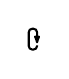
\begin{tikzpicture}[x=1.75ex,y=1.75ex,inner sep=0pt,outer sep=0pt]
    \coordinate (split) at (0,0.7);
    \begin{scope}[line width=0.175ex,rounded corners=0.3ex]
      \draw[-{Latex[round,length=1.0ex,width=0.6ex]}] (0.2,0.2) -- (0.2,0.0) -- (-0.2,0.0) -- (-0.2,1.0) -- (0.2,1.0) -- (0.2,0.3);
    \end{scope}
  \end{tikzpicture}}

\newcommand{\nonlinearCF}{
  
\begin{tikzpicture}[x=2ex,y=3ex,inner sep=0pt,outer sep=0pt,baseline={([yshift=-.75ex]current bounding box.center)}]
    \fill[nonlinear,rounded corners=2pt] (0,0) rectangle (1,1);
    \node[nonlinear!25] at (0.55,0.5) {\nonlinearCFarrow};
  \end{tikzpicture}}

\newsavebox{\linearCFbox}\savebox{\linearCFbox}{\linearCF}
\newsavebox{\nonlinearCFbox}\savebox{\nonlinearCFbox}{\nonlinearCF}
\newsavebox{\branchingCFbox}\savebox{\branchingCFbox}{\branchingCF}

\newcommand{\circled}[1]{
  \begin{tikzpicture}[outer sep=0pt,inner sep=0pt,baseline={(circ.base)}]
    \node[circle,draw=.,fill=.!25,inner sep=0.2ex,line width=0.2ex,anchor=base] (circ) {#1};
  \end{tikzpicture}
}

\newcommand{\cfoption}[2]{\hspace{-0.4em}\mbox{\bfseries\ttfamily\color{#1}\smaller\circled{#2}}\hspace{-0.4em}}
